% fig_per.tex - Plan-Execute-Reflect architecture (vertical flow, standalone -> PDF)
\documentclass[tikz,border=6pt]{standalone}
\usepackage{tikz}
\usetikzlibrary{arrows.meta,positioning,fit,backgrounds,calc,shapes.geometric}
\definecolor{ours}{HTML}{C0392B}
\definecolor{slate}{HTML}{2C3E50}
\definecolor{teal}{HTML}{16A085}
\definecolor{blue}{HTML}{2980B9}
\definecolor{lg}{HTML}{ECF0F1}
\definecolor{mgd}{HTML}{7F8C8D}
\begin{document}
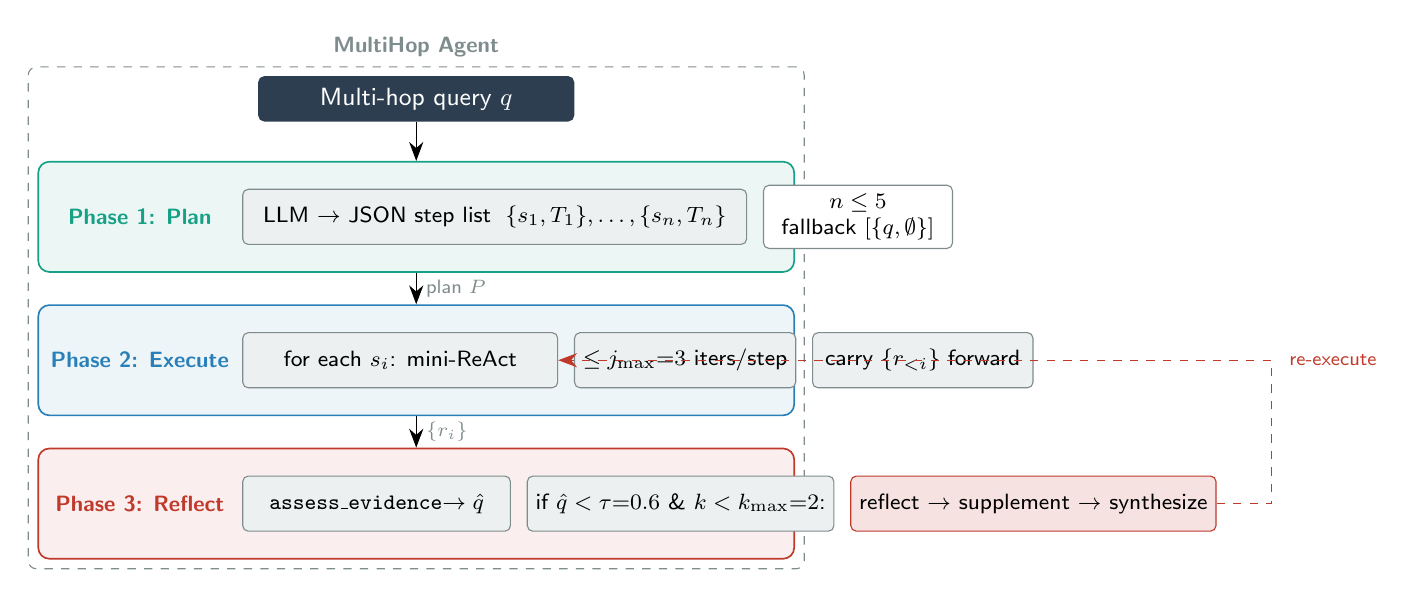
\begin{tikzpicture}[
  font=\small\sffamily,
  >={Stealth[length=2.4mm]},
  node distance=4mm and 6mm,
  phase/.style={draw=slate, rounded corners=4pt, align=center, inner sep=5pt,
                minimum width=96mm, minimum height=14mm, fill=white, line width=0.6pt},
  pbox/.style={draw=mgd, rounded corners=2pt, align=center, inner sep=3pt,
               fill=lg, line width=0.4pt, font=\footnotesize\sffamily,
               minimum height=7mm},
  plbl/.style={font=\footnotesize\sffamily\bfseries},
]
% query
\node[draw=slate, fill=slate, text=white, rounded corners=2pt, inner sep=4pt,
      minimum width=40mm] (q) {Multi-hop query $q$};

% Phase 1: Plan
\node[phase, below=5mm of q, fill=teal!8, draw=teal] (p1) {};
\node[plbl, color=teal] at ($(p1.west)+(13mm,0)$) {Phase 1: Plan};
\node[pbox, right=2mm of p1.west, xshift=24mm, minimum width=64mm] (llm1)
  {LLM $\to$ JSON step list \;$\{s_1,T_1\},\ldots,\{s_n,T_n\}$};
\node[pbox, right=2mm of llm1, minimum width=24mm, fill=white] (bnd)
  {$n\leq 5$\\fallback $[\{q,\emptyset\}]$};

% Phase 2: Execute
\node[phase, below=4mm of p1, fill=blue!8, draw=blue] (p2) {};
\node[plbl, color=blue] at ($(p2.west)+(13mm,0)$) {Phase 2: Execute};
\node[pbox, right=2mm of p2.west, xshift=24mm, minimum width=40mm] (step)
  {for each $s_i$: mini-ReAct};
\node[pbox, right=2mm of step, minimum width=28mm] (react)
  {$\leq j_{\max}{=}3$ iters/step};
\node[pbox, right=2mm of react, minimum width=28mm] (flow)
  {carry $\{r_{<i}\}$ forward};

% Phase 3: Reflect & Synthesize
\node[phase, below=4mm of p2, fill=ours!8, draw=ours] (p3) {};
\node[plbl, color=ours] at ($(p3.west)+(13mm,0)$) {Phase 3: Reflect};
\node[pbox, right=2mm of p3.west, xshift=24mm, minimum width=34mm] (ass)
  {\texttt{assess\_evidence}$\to\hat q$};
\node[pbox, right=2mm of ass, minimum width=30mm] (chk)
  {if $\hat q<\tau{=}0.6$ \& $k<k_{\max}{=}2$:};
\node[pbox, right=2mm of chk, minimum width=26mm, fill=ours!14, draw=ours] (syn)
  {reflect $\to$ supplement $\to$ synthesize};

% edges
\draw[->] (q) -- (p1);
\draw[->] (p1) -- node[right, font=\scriptsize\sffamily, color=mgd]{plan $P$} (p2);
\draw[->] (p2) -- node[right, font=\scriptsize\sffamily, color=mgd]{$\{r_i\}$} (p3);
% reflect loop back to Execute
\draw[->, ours, dashed] (syn.east) -- ++(7mm,0) |- (step.east)
  node[midway, right, font=\scriptsize\sffamily, color=ours, xshift=1mm]
  {re-execute};

\begin{scope}[on background layer]
  \node[draw=mgd, dashed, rounded corners=3pt, fit=(q)(p1)(p2)(p3),
        label={[font=\footnotesize\sffamily\bfseries,color=mgd]above:MultiHop Agent}] {};
\end{scope}
\end{tikzpicture}
\end{document}
